% QWEN-ARCHITECTURE REVIEW POSTER (2026-10-19). Derived from poster_visual_final_review.tex under the user's addendum
% "ARC SUMMIT POSTER: MAKE THE QWEN-CORA IDEA VISIBLE" and the later instruction "use at most a small dashed
% future-direction diagram on the poster". For collaborator review (Toni, Chris, Pierce); NOT for print until approved.
% poster_visual_final_review.* and docs/summit_poster/poster.pdf are unchanged.
% Numbers: records/CORA_SUMMIT_CLAIM_LEDGER_20261017.md (audited in POSTER_CLAIM_AUDIT.md; new statements in
% POSTER_QWEN_ARCHITECTURE_NOTES.md). Figures: figures/ (scripts/summit_visual_figures.py, hash-pinned inputs;
% provenance in figures/PROVENANCE.json). Illustrative figures say so on their face.
% Diagrams: TikZ. Solid outline = existing and tested; dashed = proposed, not implemented or validated.
% Size: A0 portrait is a REVIEW ASSUMPTION (no organizer guide on file). Body 30 pt; diagram text 22-26 pt; figure text >= 20 pt.
% Build: SOURCE_DATE_EPOCH=1791763200 FORCE_SOURCE_DATE=1 pdflatex poster_qwen_architecture_review.tex (POSTER_QWEN_ARCHITECTURE_NOTES.md).
\RequirePackage{fix-cm}
\documentclass[25pt, a0paper, portrait, blockverticalspace=7mm]{tikzposter}
\usepackage[scaled]{helvet}
\renewcommand{\familydefault}{\sfdefault}
\usepackage[T1]{fontenc}
\usepackage{graphicx}
\usepackage{enumitem}
\usepackage{array}
\usepackage{amssymb}
\usetikzlibrary{positioning, arrows.meta, fit, calc, shapes.geometric}
\pdftrailerid{}
\hyphenpenalty=10000
\exhyphenpenalty=10000

\newcommand{\bodyfont}{\fontsize{30}{38}\selectfont\raggedright}
\newcommand{\secfont}{\fontsize{26}{32}\selectfont\raggedright}
\newcommand{\diagfont}{\fontsize{26}{31}\selectfont}
\newcommand{\diagsub}{\fontsize{22}{27}\selectfont}
\newcommand{\bignum}[1]{{\fontsize{120}{120}\selectfont\bfseries #1}}
\newcommand{\bt}[1]{{\fontsize{40}{48}\selectfont #1}}
\newcommand{\chip}[2]{{\fontsize{26}{30}\selectfont\color{#1}\,[#2]}}
\setlist{leftmargin=1.1em, itemsep=0.2em, topsep=0.2em, parsep=0pt}

\definecolor{ink}{HTML}{0B0B0B}
\definecolor{ink2}{HTML}{52514E}
\definecolor{accent}{HTML}{2A78D6}
\definecolor{warm}{HTML}{EB6834}
\definecolor{good}{HTML}{0CA30C}
\definecolor{neutral}{HTML}{F0EFEC}
\definecolor{critical}{HTML}{D03B3B}
\definecolor{paper}{HTML}{FCFCFB}
\definecolor{arcblue}{HTML}{0074D9}
\definecolor{arcred}{HTML}{FF4136}

\usetheme{Simple}
\tikzposterlatexaffectionproofoff
\colorlet{backgroundcolor}{paper}
\colorlet{framecolor}{paper}
\colorlet{titlefgcolor}{ink}
\colorlet{titlebgcolor}{paper}
\colorlet{blocktitlebgcolor}{paper}
\colorlet{blocktitlefgcolor}{accent}
\colorlet{blockbodybgcolor}{paper}
\colorlet{blockbodyfgcolor}{ink}
\makeatletter
\settitle{\centering\vbox{\color{titlefgcolor}{\bfseries\fontsize{100}{112}\selectfont \@title\par}\vspace*{0.2em}%
  {\fontsize{52}{62}\selectfont \@author\par}\vspace*{0.25em}{\fontsize{36}{44}\selectfont\color{ink2} \@institute}}}
\makeatother

\title{LEARNING WHAT TO CHANGE}
\author{From Visual Reasoning to Scientific Hypothesis Revision}
\institute{Chimdi Walter Ndubuisi \,$\cdot$\, University of Missouri \quad {\color{critical}REVIEW DRAFT 19 October: for collaborator review, not for print}}

\tikzset{
  stage/.style={rounded corners=8pt, draw=accent, line width=2.6pt, fill=white, align=center, font=\diagfont,
                inner sep=9pt},
  pstage/.style={stage, dashed, draw=ink2, dash pattern=on 12pt off 7pt},
  test/.style={stage, draw=ink, line width=3.4pt, fill=neutral},
  flow/.style={-{Latex[length=8mm,width=6mm]}, line width=2.8pt, draw=ink2},
  lab/.style={font=\diagsub, text=ink2, align=center},
}

\begin{document}
\maketitle[width=0.97\linewidth]

%======================= THE CENTRAL QUESTION (full width)
\block{}{%
  \centering
  {\fontsize{58}{68}\selectfont\bfseries Can a reasoner recognize when its explanation is inadequate,\\[0.1em]
   and determine what needs to change?\par}
  \vspace{0.35em}
  {\fontsize{30}{37}\selectfont\color{ink2} Find what is missing, choose a revision, test it. A question shaped in
   discussions with Toni Kazic.\par}
}

\begin{columns}

%======================= COLUMN 1: why reasoning fails
\column{0.333}
\block{\bt{1 \;$\cdot$\; Why reasoning fails}}{\bodyfont
  One rule must fit both examples and the new input.
  \begin{tikzfigure}
    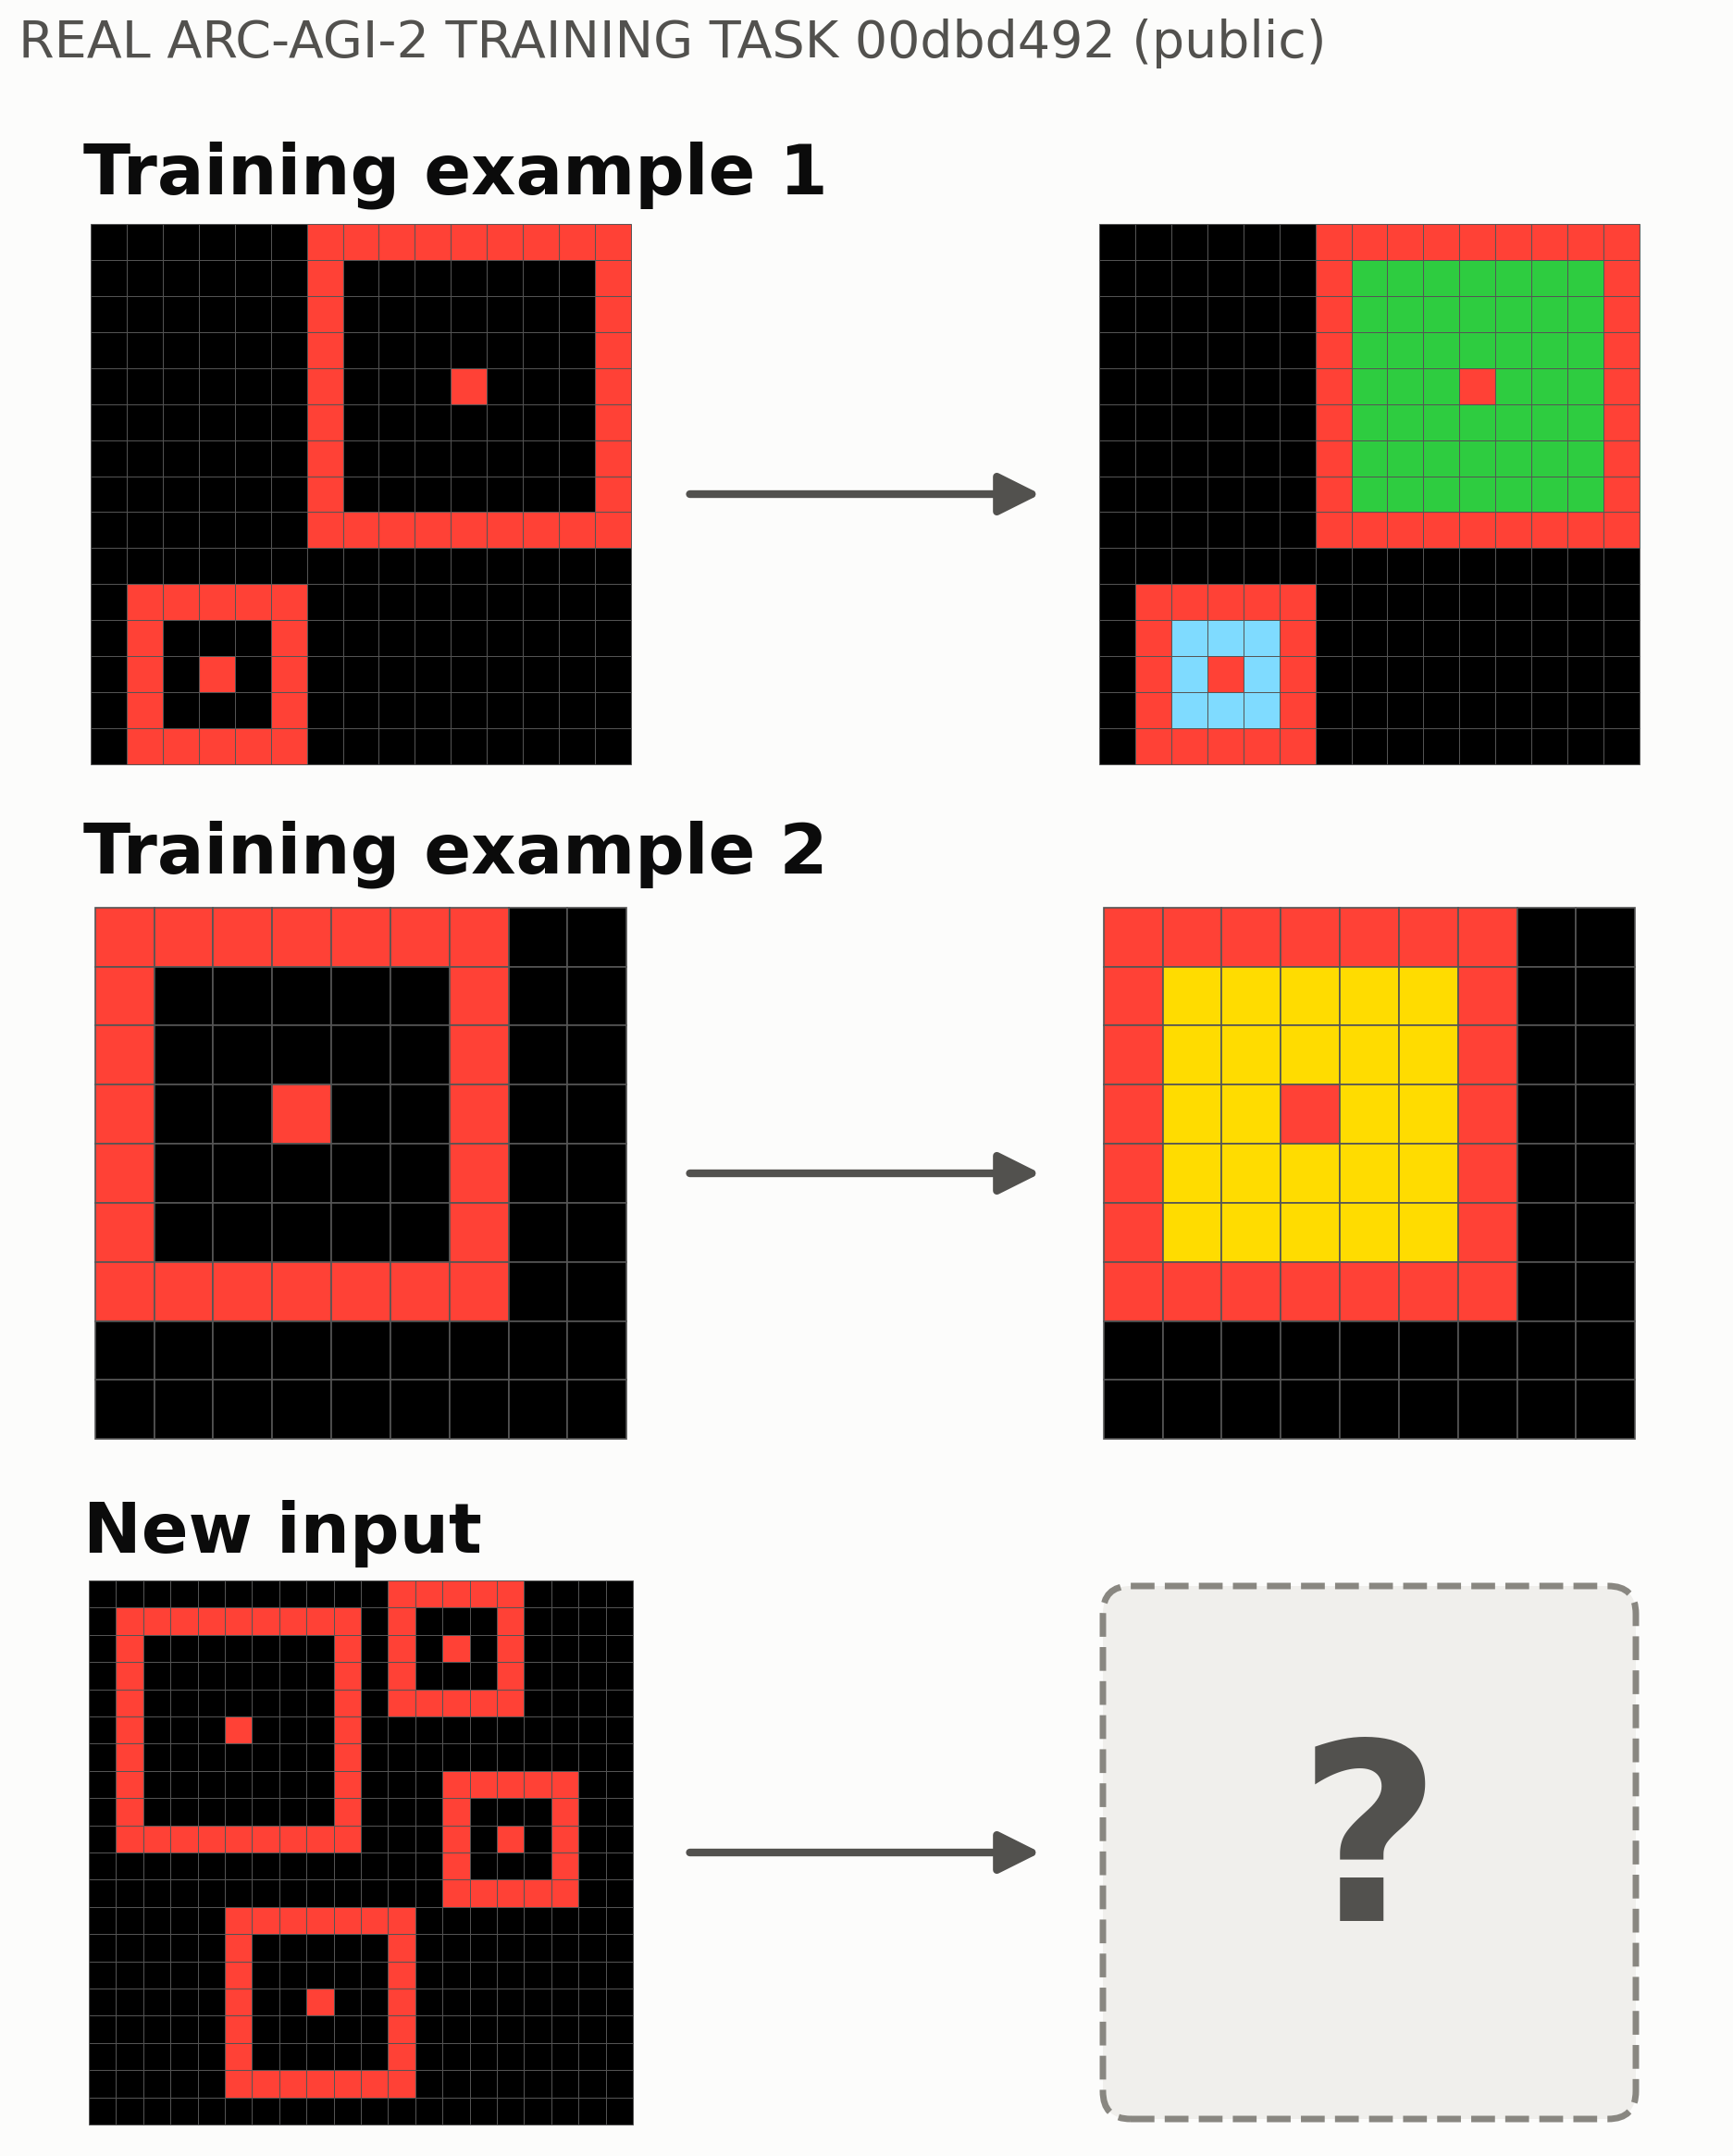
\includegraphics[width=\linewidth]{figures/fig_arc_intro_00dbd492_large.png}
  \end{tikzfigure}
  \secfont\color{ink2} Rule: each frame's fill colour depends on its size.
}
\block{\bt{Three ways an explanation fails}}{\bodyfont
  \begin{tikzfigure}
    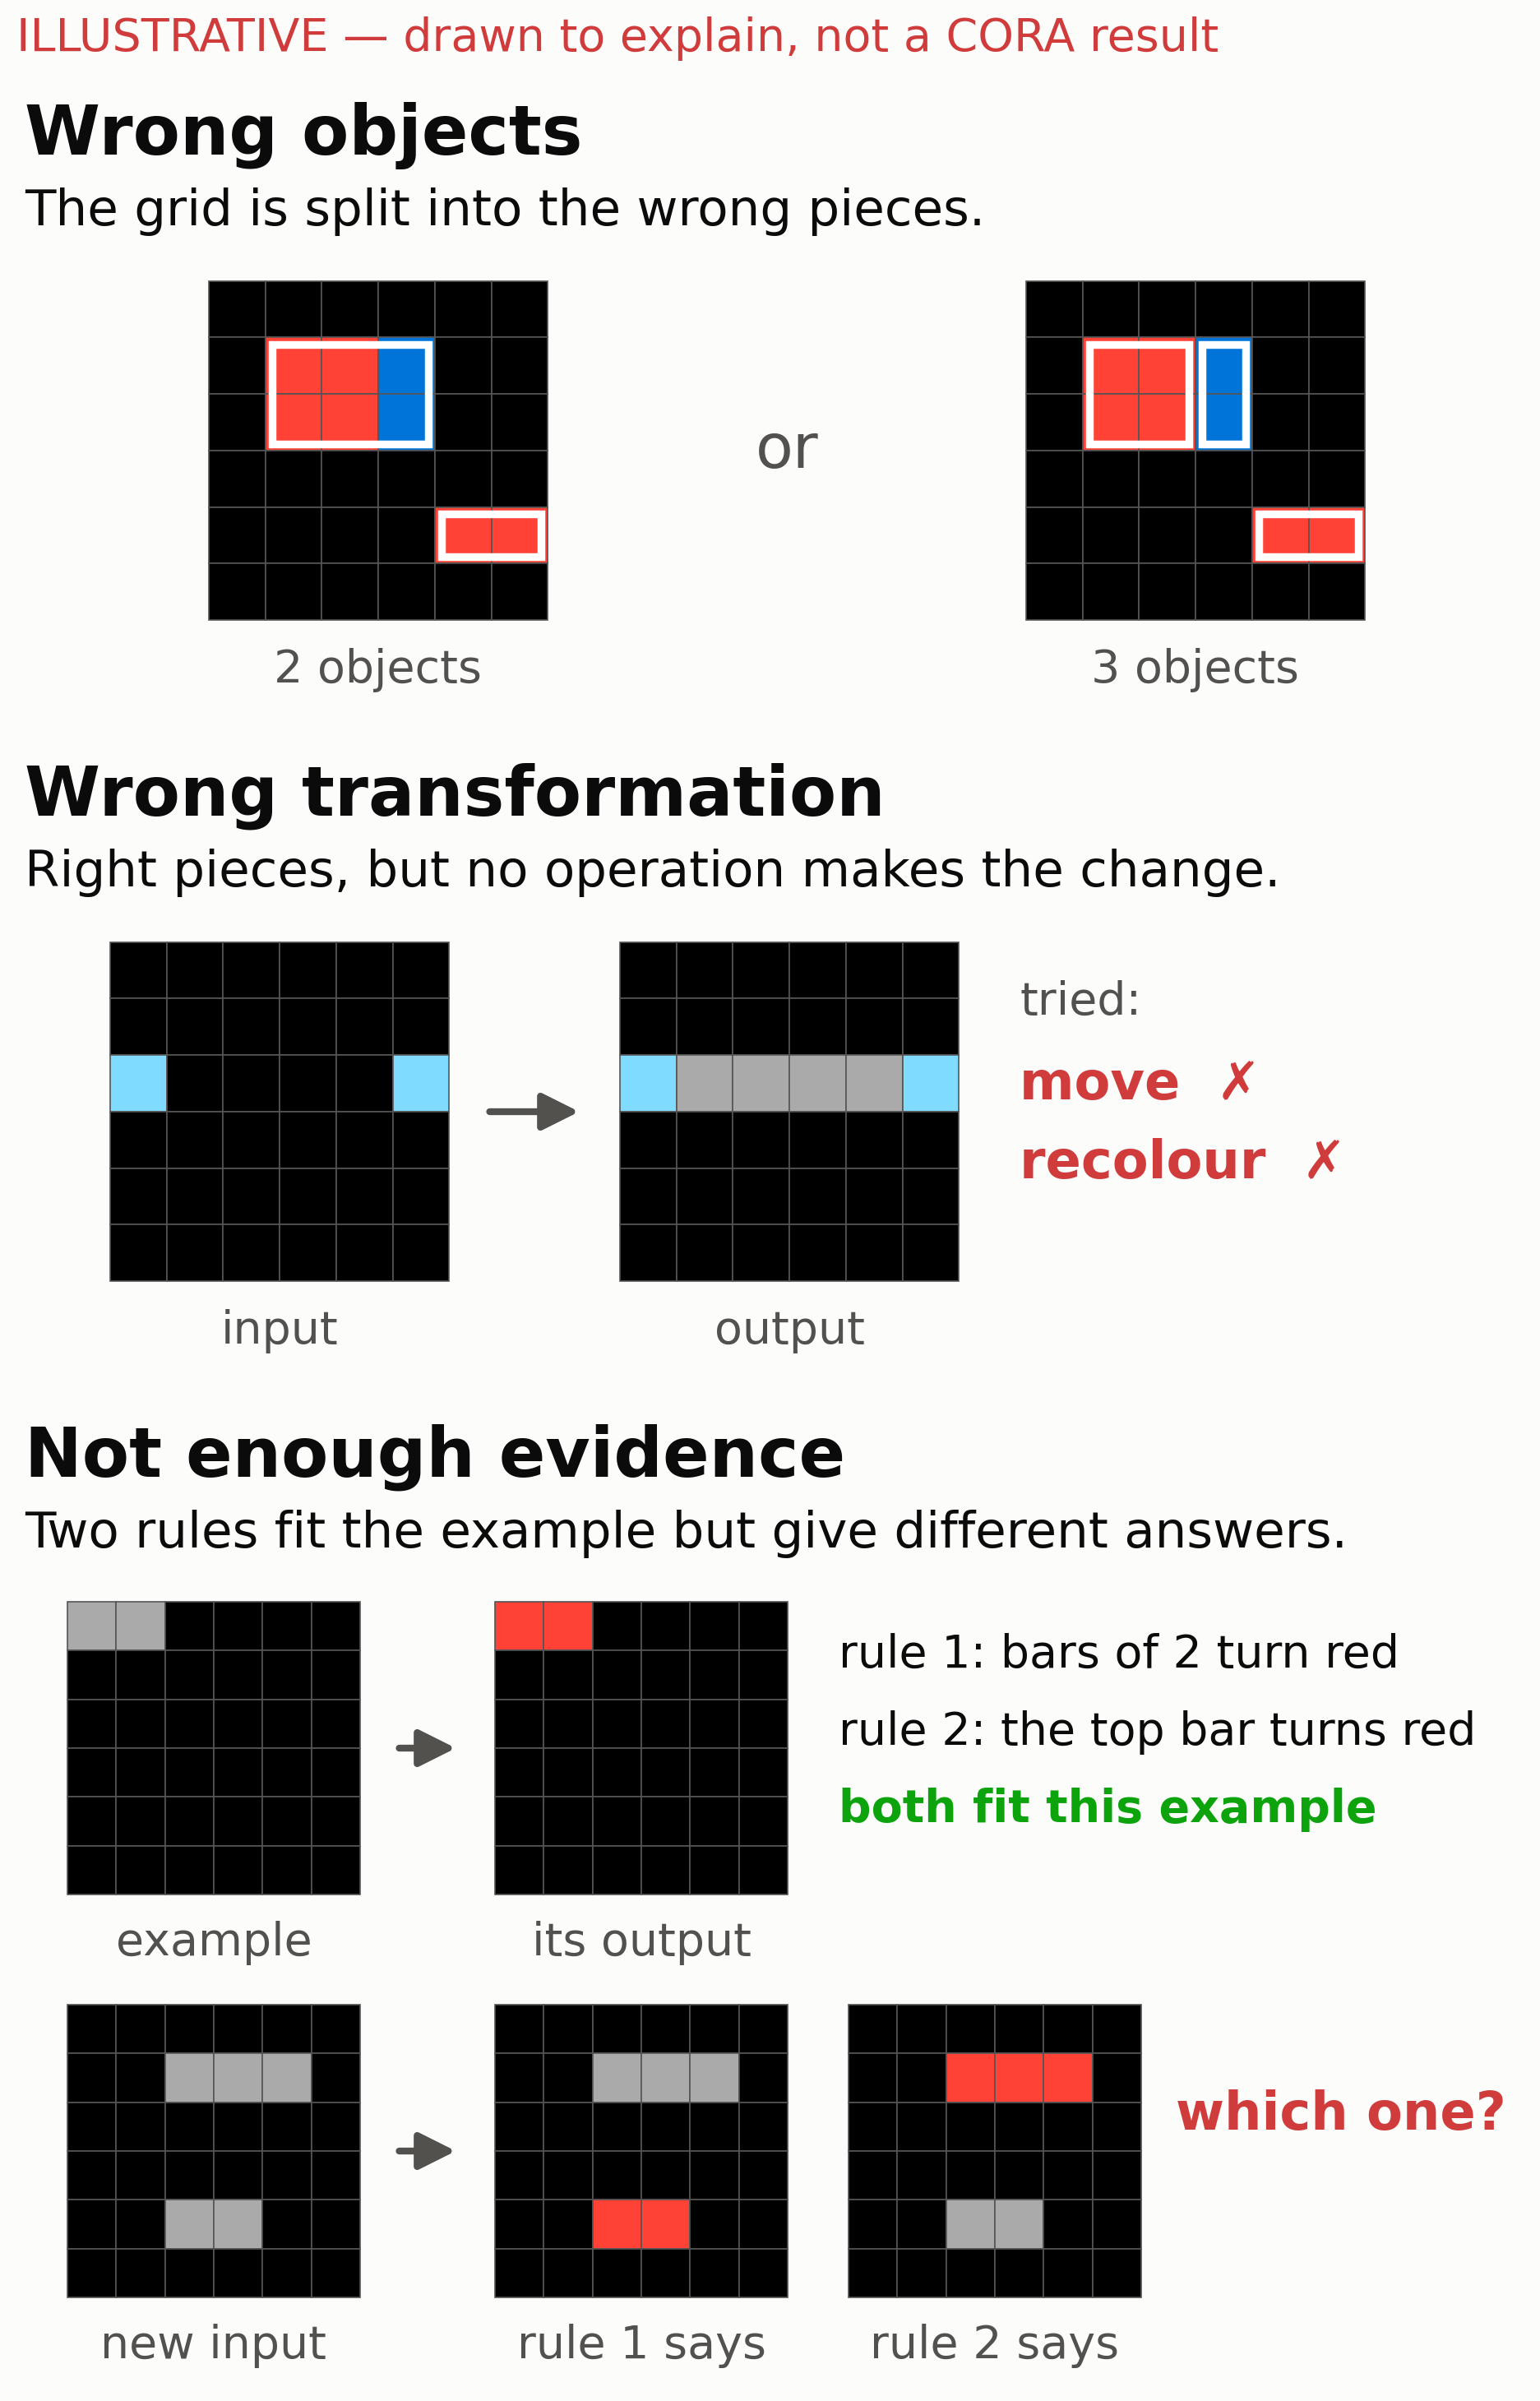
\includegraphics[width=\linewidth]{figures/fig_three_failures_ILLUSTRATIVE.png}
  \end{tikzfigure}
  Telling these apart is the research problem.
}

%======================= COLUMN 2: what CORA has demonstrated
\column{0.333}
\block{\bt{2 \;$\cdot$\; What CORA has demonstrated}}{\bodyfont
  CORA writes rules as programs.
}
\block{\bt{Fitting is not enough}\chip{good}{DONE}}{\bodyfont
  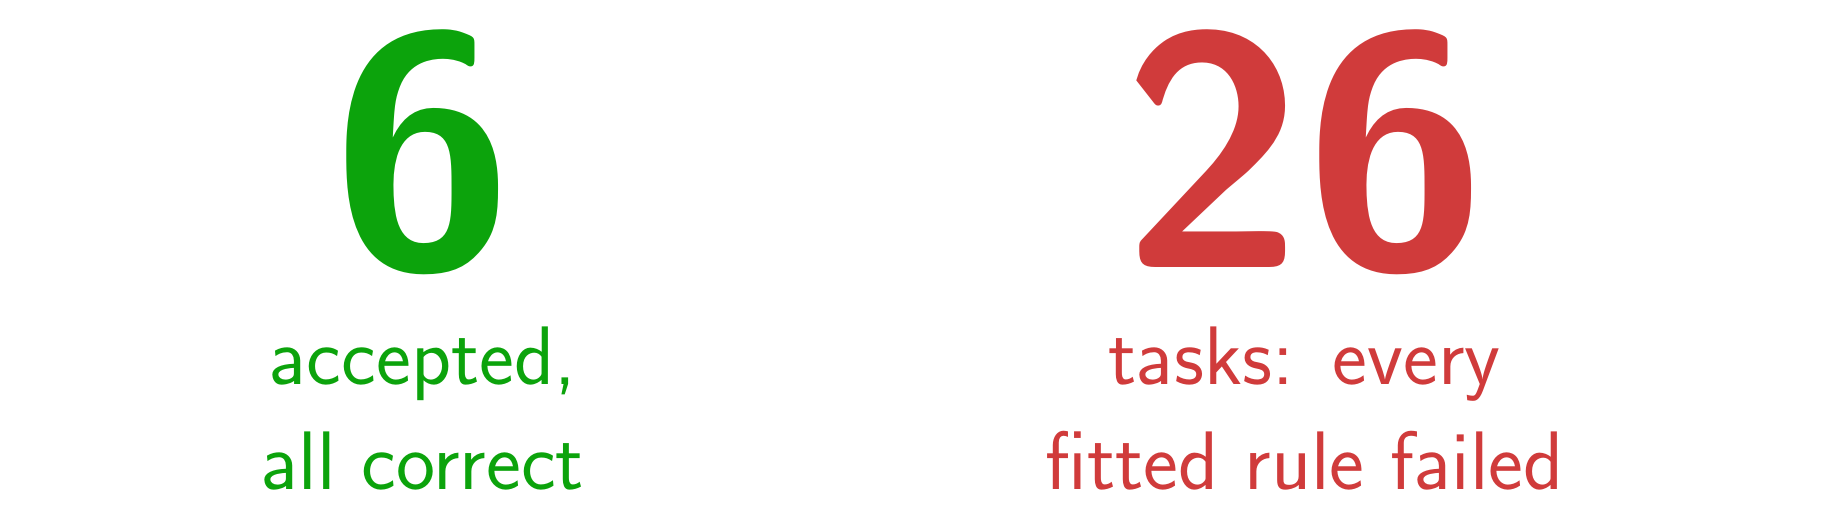
\begin{tikzpicture}
    \node[anchor=north, text width=9.8cm, align=center, font=\fontsize{30}{38}\selectfont] at (0,0)
      {\color{good}\bignum{6}\\[0.15em] accepted,\\ all correct};
    \node[anchor=north, text width=12.2cm, align=center, font=\fontsize{30}{38}\selectfont] at (11.2,0)
      {\color{critical}\bignum{26}\\[0.15em] tasks: every\\ fitted rule failed};
  \end{tikzpicture}
  \par\secfont\color{ink2} 60 exposed training tasks.
}
\block{\bt{A rule CORA built}\chip{good}{DONE, NARROW}}{\bodyfont
  \begin{tikzfigure}
    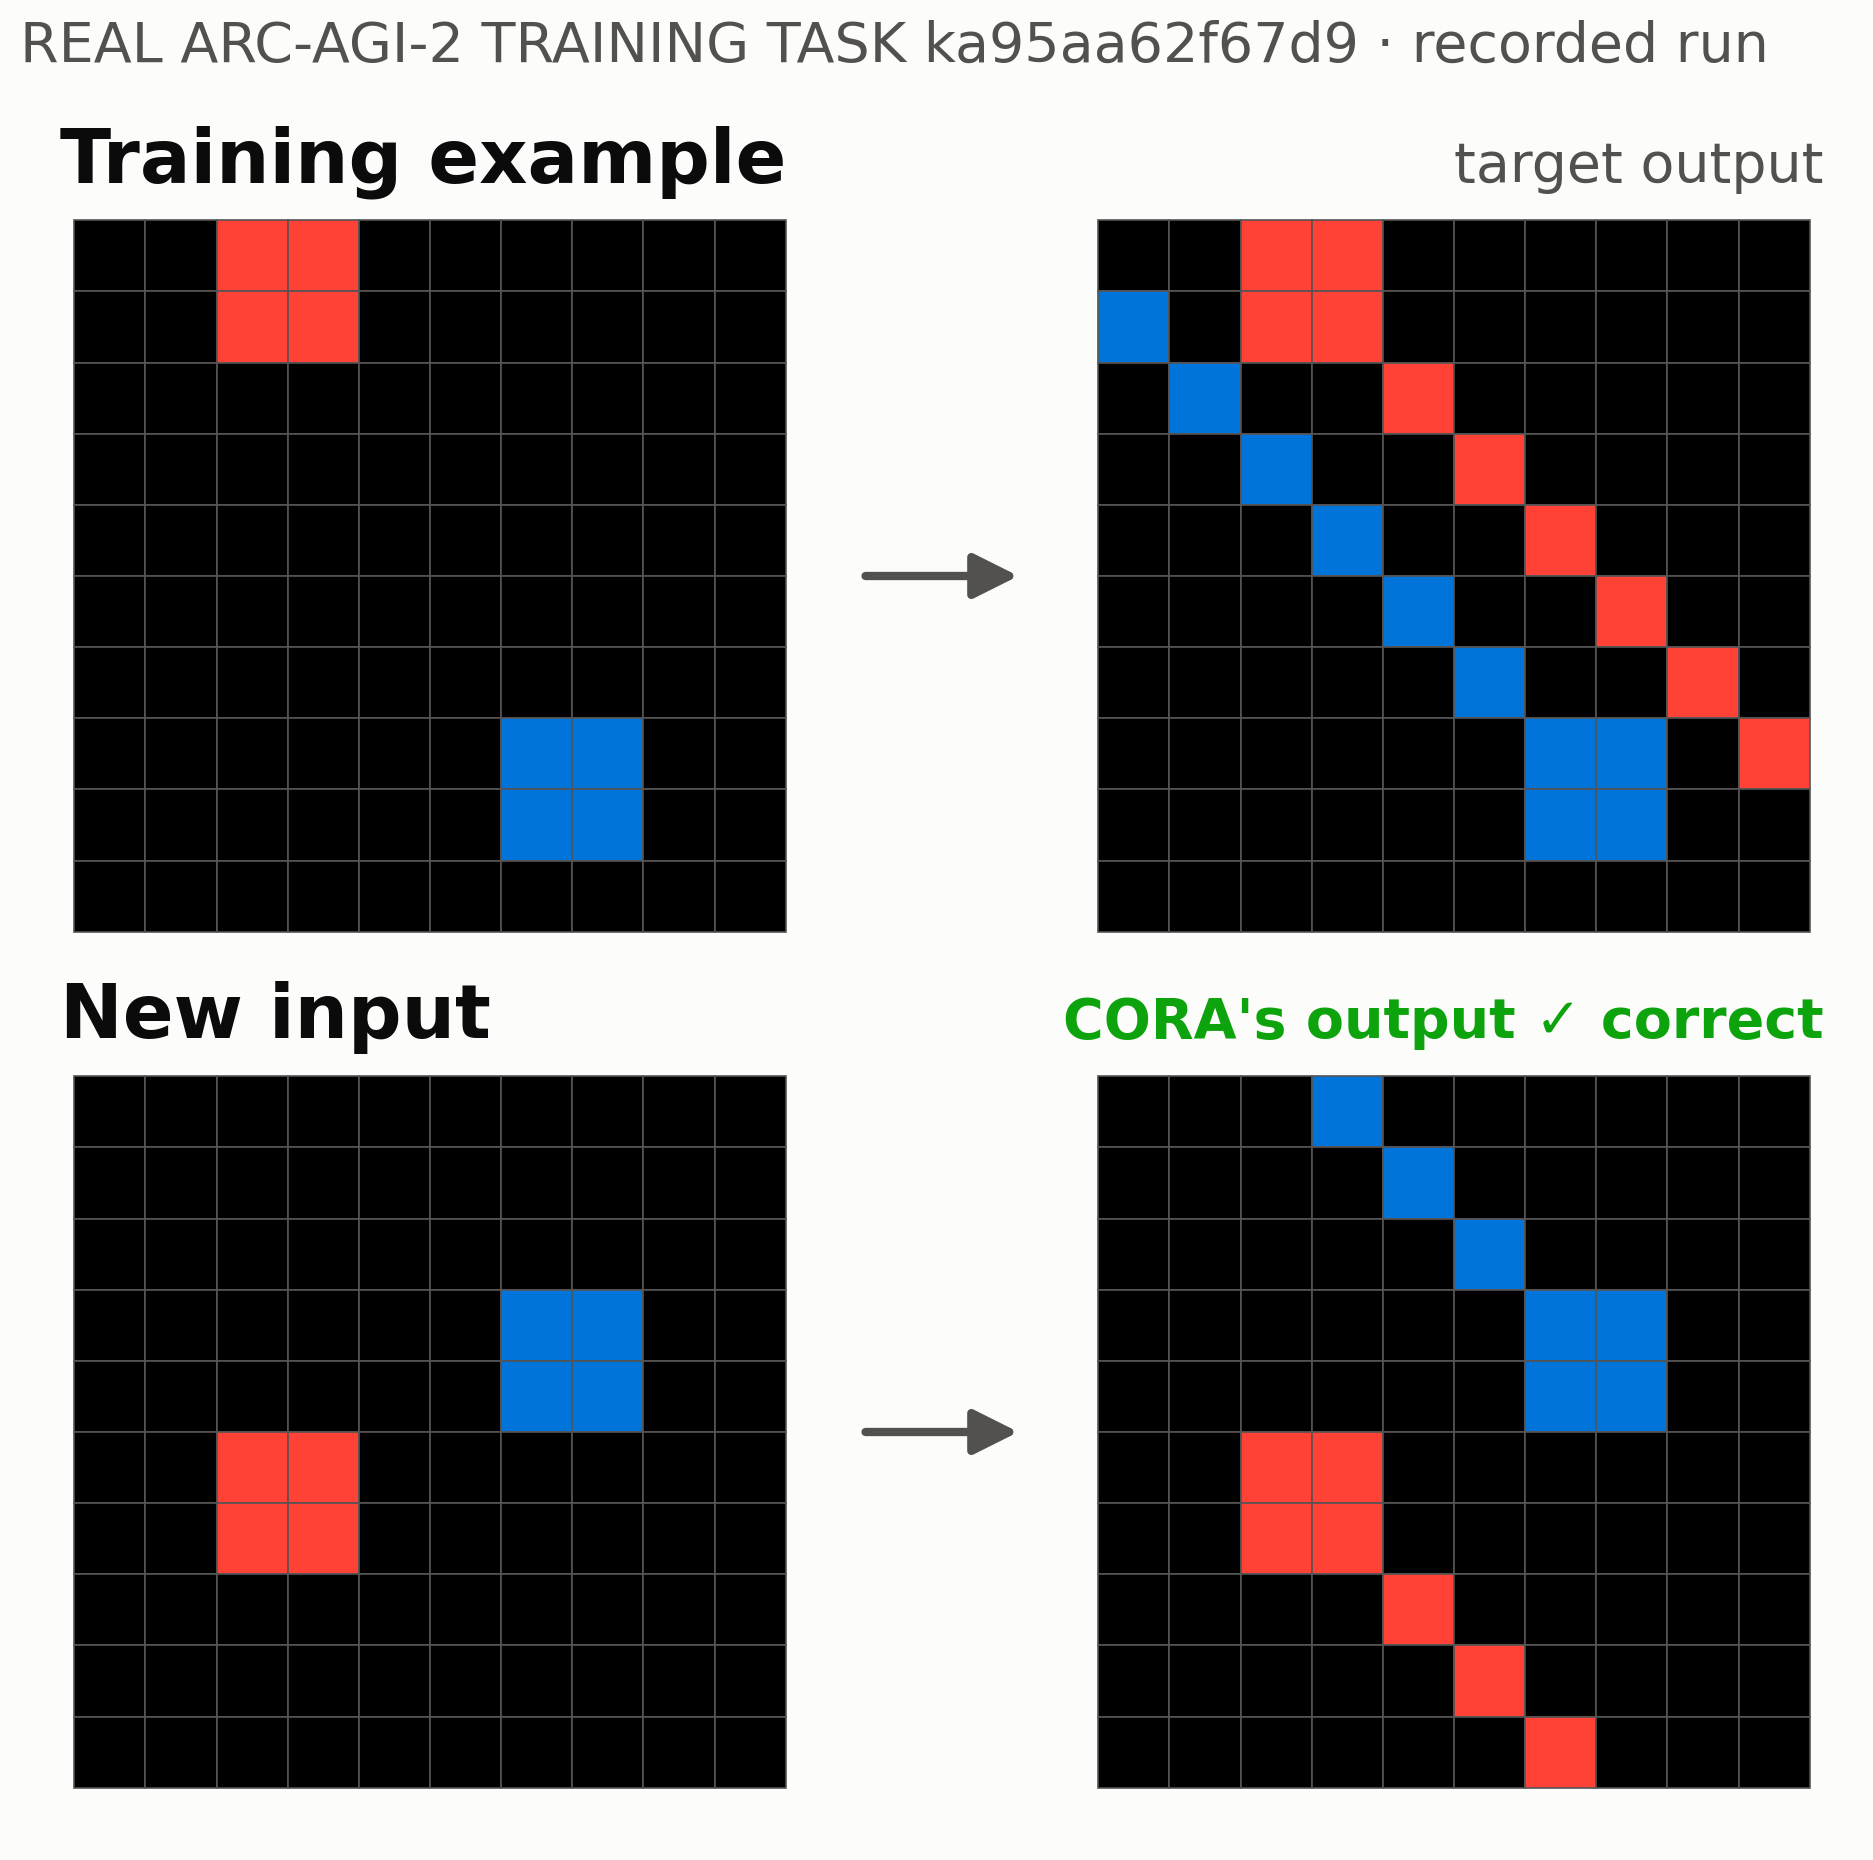
\includegraphics[width=\linewidth]{figures/fig_real_rule_ka95aa62f67d9_large.png}
  \end{tikzfigure}
  \textbf{Rule:} {\color{arcblue}\textbf{blue}} objects send a line up-left; {\color{arcred}\textbf{red}} ones,
  down-right.
  \begin{itemize}[leftmargin=1.5cm, labelsep=0.45cm, itemsep=0.1em, topsep=0.35em]
    \secfont
    \item[\textcolor{good}{$\checkmark$}] constructed by CORA
    \item[\textcolor{good}{$\checkmark$}] correct on this task
    \item[\textcolor{good}{$\checkmark$}] rebuilt 3 of 3 times, one example hidden
    \item[\textcolor{ink2}{\textbf{=}}] also found without the failure record
  \end{itemize}
  \secfont\color{ink2}\textbf{An exposed training task, not a Kaggle success.}
}
\block{\bt{Did it generalize?}\chip{critical}{NEGATIVE}}{\bodyfont
  \centering{\color{critical}\bignum{0 / 58}}\par\vspace{0.1em}
  new verified solutions\par\vspace{0.2em}
  \begin{tikzfigure}
    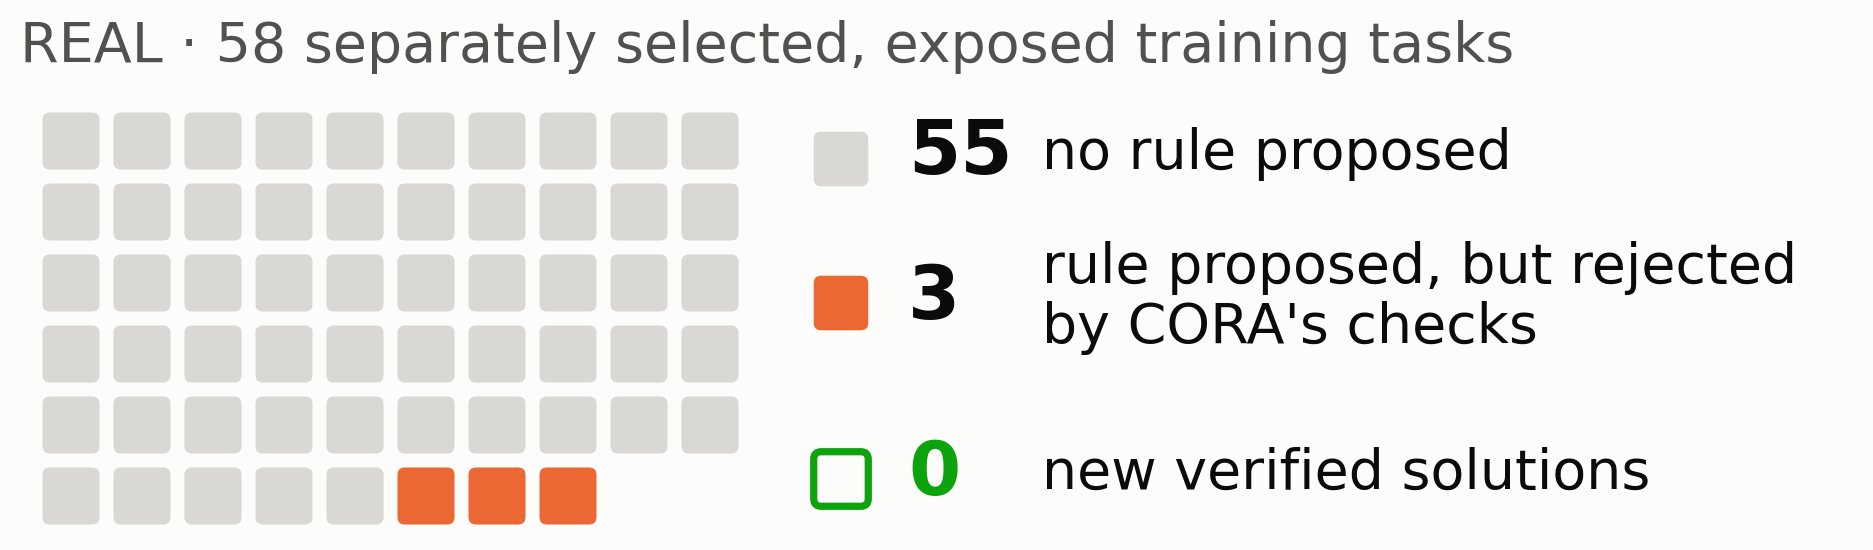
\includegraphics[width=\linewidth]{figures/fig_construction_58_outcomes.png}
  \end{tikzfigure}
  \raggedright\secfont\color{ink2} Every variant found 0; no wrong answers.
}

%======================= COLUMN 3: how neural learning may help
\column{0.333}
\block{\bt{3 \;$\cdot$\; How neural learning may help}}{\bodyfont
  \begin{tikzfigure}
  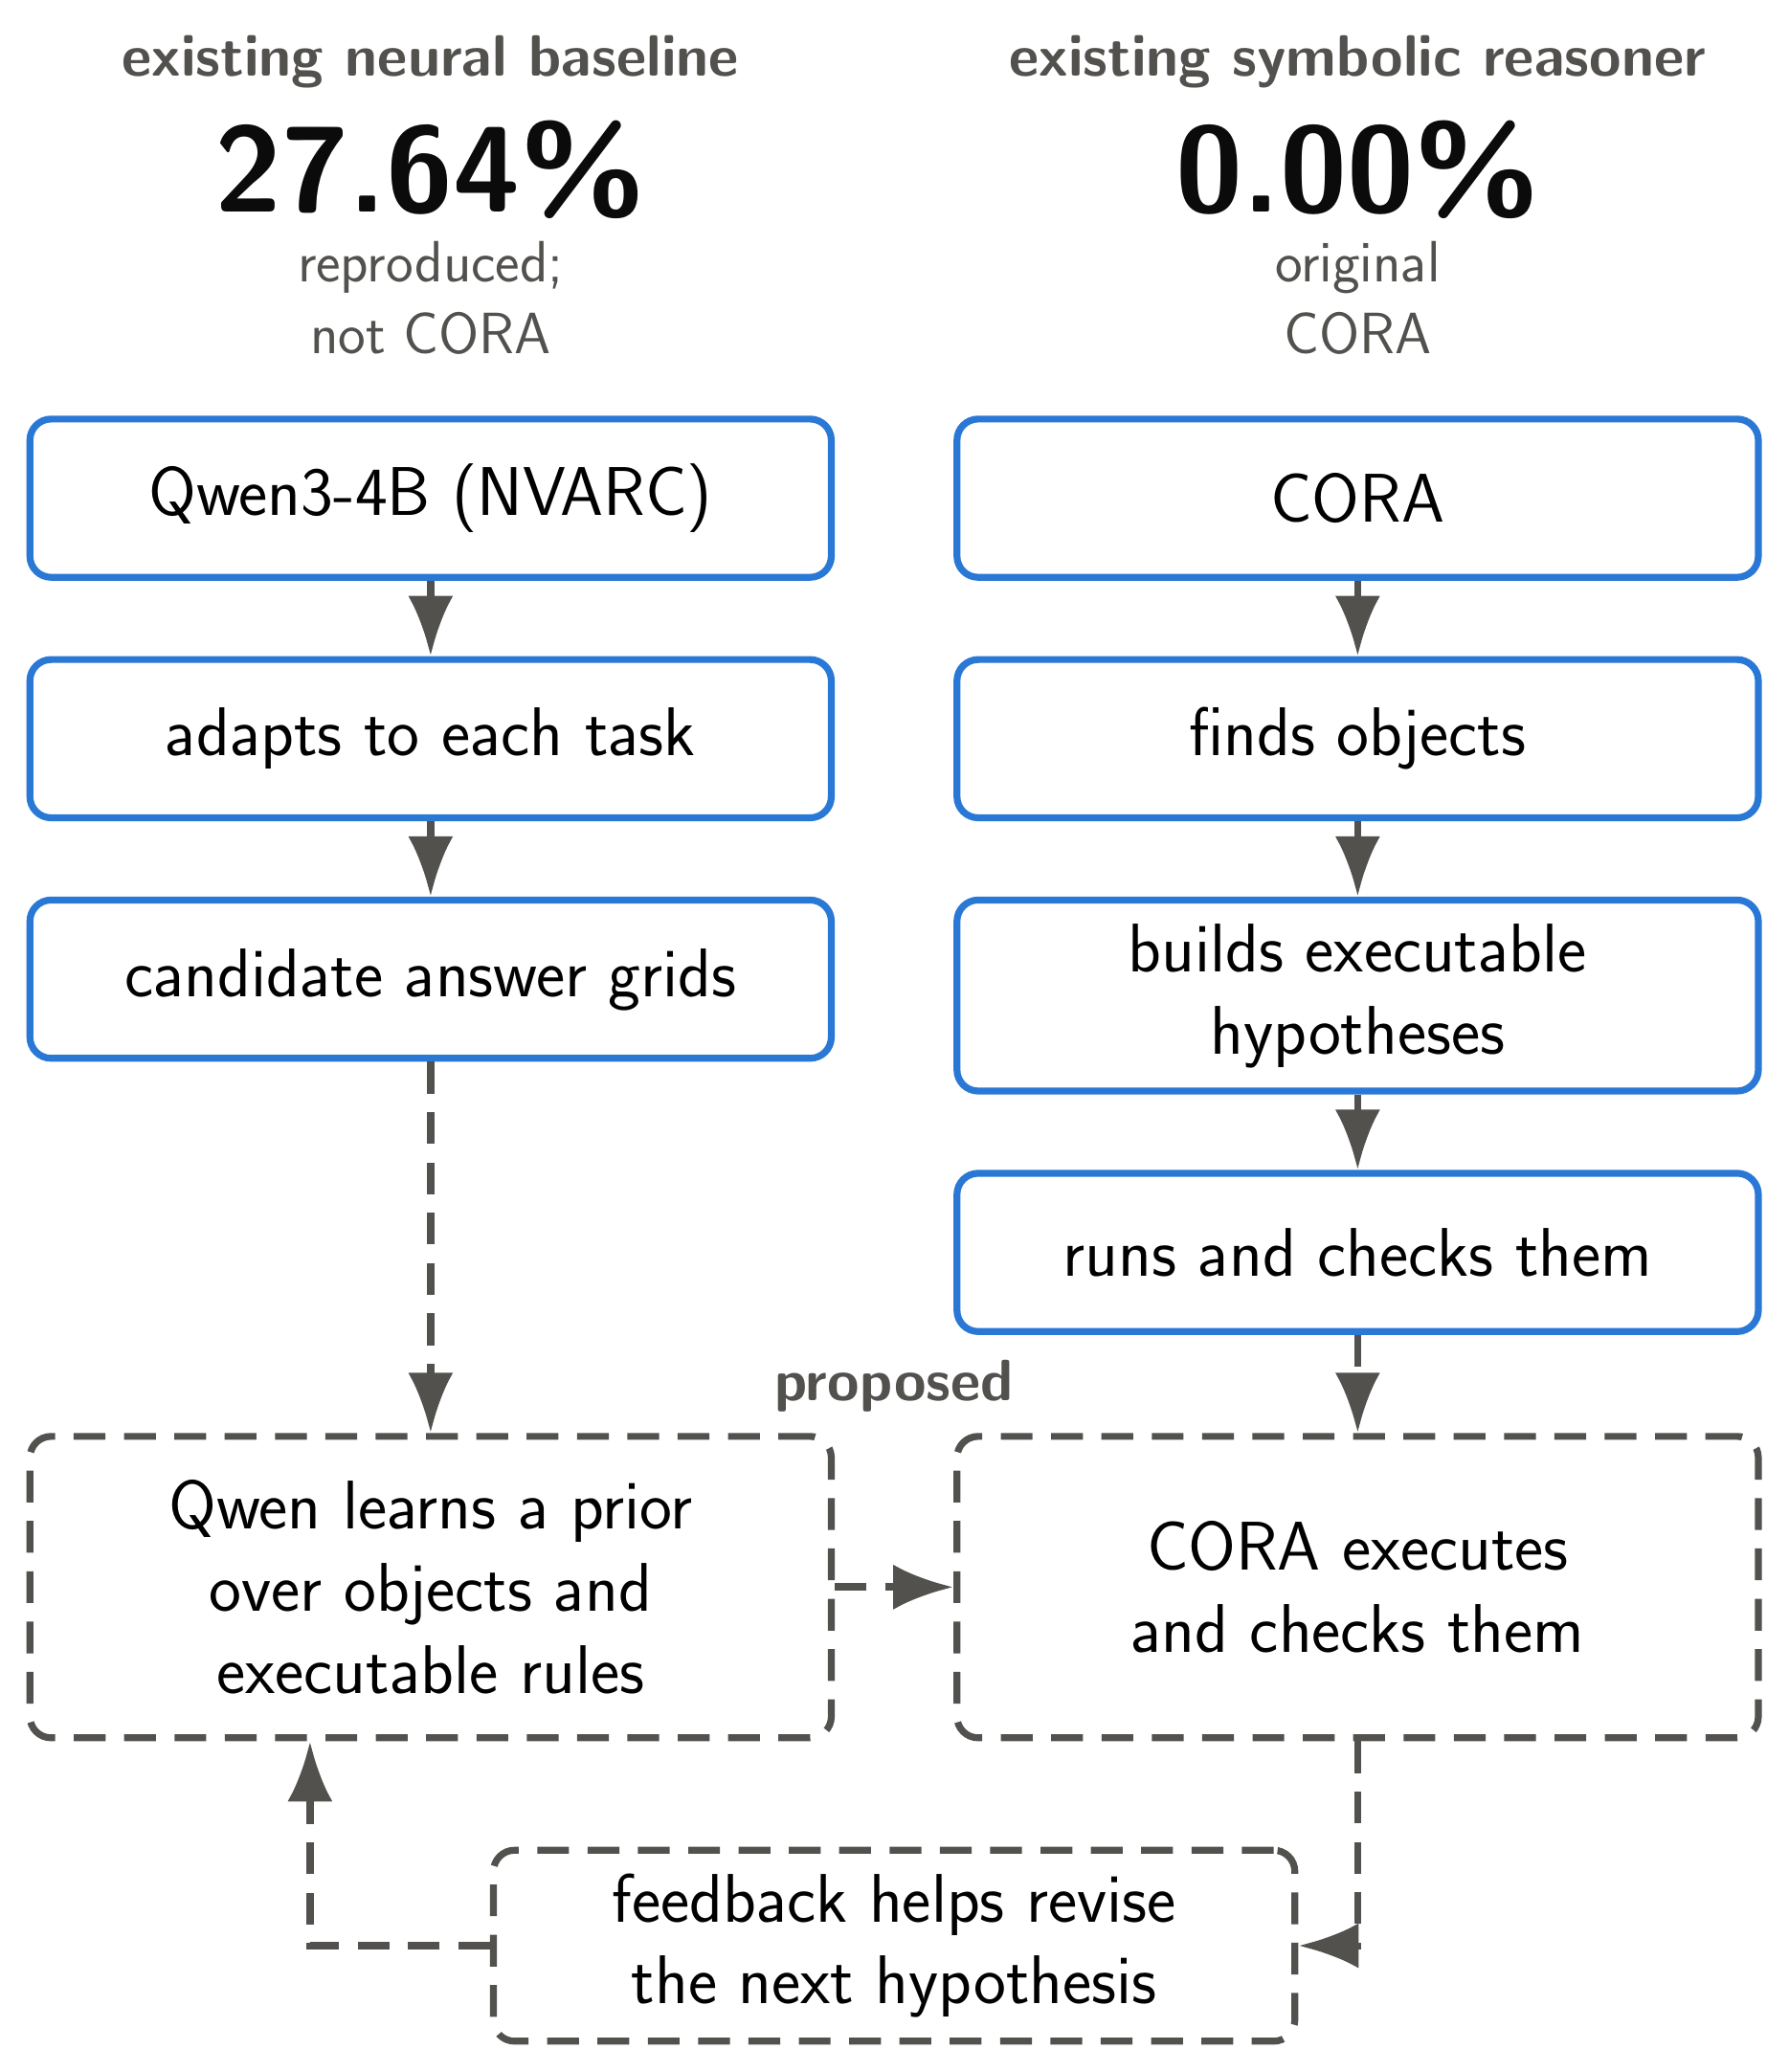
\begin{tikzpicture}[
      lane/.style={stage, text width=10.0cm, minimum height=2.1cm},
      wide/.style={pstage, text width=19.6cm, minimum height=2.1cm},
      dflow/.style={flow, dashed, dash pattern=on 12pt off 7pt},
      lanehead/.style={font=\diagsub\bfseries, text=ink2},
      score/.style={font=\fontsize{46}{50}\selectfont\bfseries, text=ink},
    ]
    \coordinate (o) at (0,0);
    \node[lanehead] (hL) at (-6.15,0) {existing neural baseline};
    \node[lanehead] (hR) at (6.15,0) {existing symbolic reasoner};
    \node[score, below=0.2cm of hL] (sL) {27.64\%};
    \node[score, below=0.2cm of hR] (sR) {0.00\%};
    \node[lab, below=0.05cm of sL] (tL) {reproduced;\\ not CORA};
    \node[lab, below=0.05cm of sR] (tR) {original\\ CORA};
    \node[lane, below=0.7cm of tL] (n1) {Qwen3-4B (NVARC)};
    \node[lane, below=1.0cm of n1] (n2) {adapts to each task};
    \node[lane, below=1.0cm of n2] (n3) {candidate answer grids};
    \node[lane, below=0.7cm of tR] (c1) {CORA};
    \node[lane, below=1.0cm of c1] (c2) {finds objects};
    \node[lane, below=1.0cm of c2] (c3) {builds executable hypotheses};
    \node[lane, below=1.0cm of c3] (c4) {runs and checks them};
    \draw[flow] (n1) -- (n2); \draw[flow] (n2) -- (n3);
    \draw[flow] (c1) -- (c2); \draw[flow] (c2) -- (c3); \draw[flow] (c3) -- (c4);
    \path (c4.south) ++(0,-1.3) coordinate (top);
    \node[pstage, text width=10.0cm, minimum height=4.0cm, anchor=north] (q1) at (n3.south |- top)
      {Qwen learns a prior over objects and executable rules};
    \node[pstage, text width=10.0cm, minimum height=4.0cm, anchor=north] (q2) at (c4.south |- top)
      {CORA executes and checks them};
    \node[pstage, text width=10.0cm, below=1.4cm of o |- q1.south, anchor=north] (q3)
      {feedback helps revise the next hypothesis};
    \node[font=\diagsub\bfseries, text=ink2] at ($(o |- top)+(0,0.62)$) {proposed};
    \draw[dflow] (n3.south) -- (q1.north);
    \draw[dflow] (c4.south) -- (q2.north);
    \draw[dflow] (q1) -- (q2);
    \draw[dflow] (q2.south) |- (q3.east);
    \draw[dflow] (q3.west) -| ([xshift=-1.6cm]q1.south);
  \end{tikzpicture}
  \end{tikzfigure}
  \textbf{Can neural learning help a reasoner discover useful representations and rules---and can executable
  verification help it determine what to change when those explanations are inadequate?}\par\vspace{0.3em}
  \secfont\color{ink2} Solid: existing. Dashed: proposed; the neural proposal interface has not yet been
  implemented or experimentally validated. Scores: official public.
}
\block{\bt{CORA-v2}\chip{warm}{DEVELOPMENT}}{\bodyfont
  Keeps all fitting rules; flags thin evidence.
  \begin{tikzfigure}
    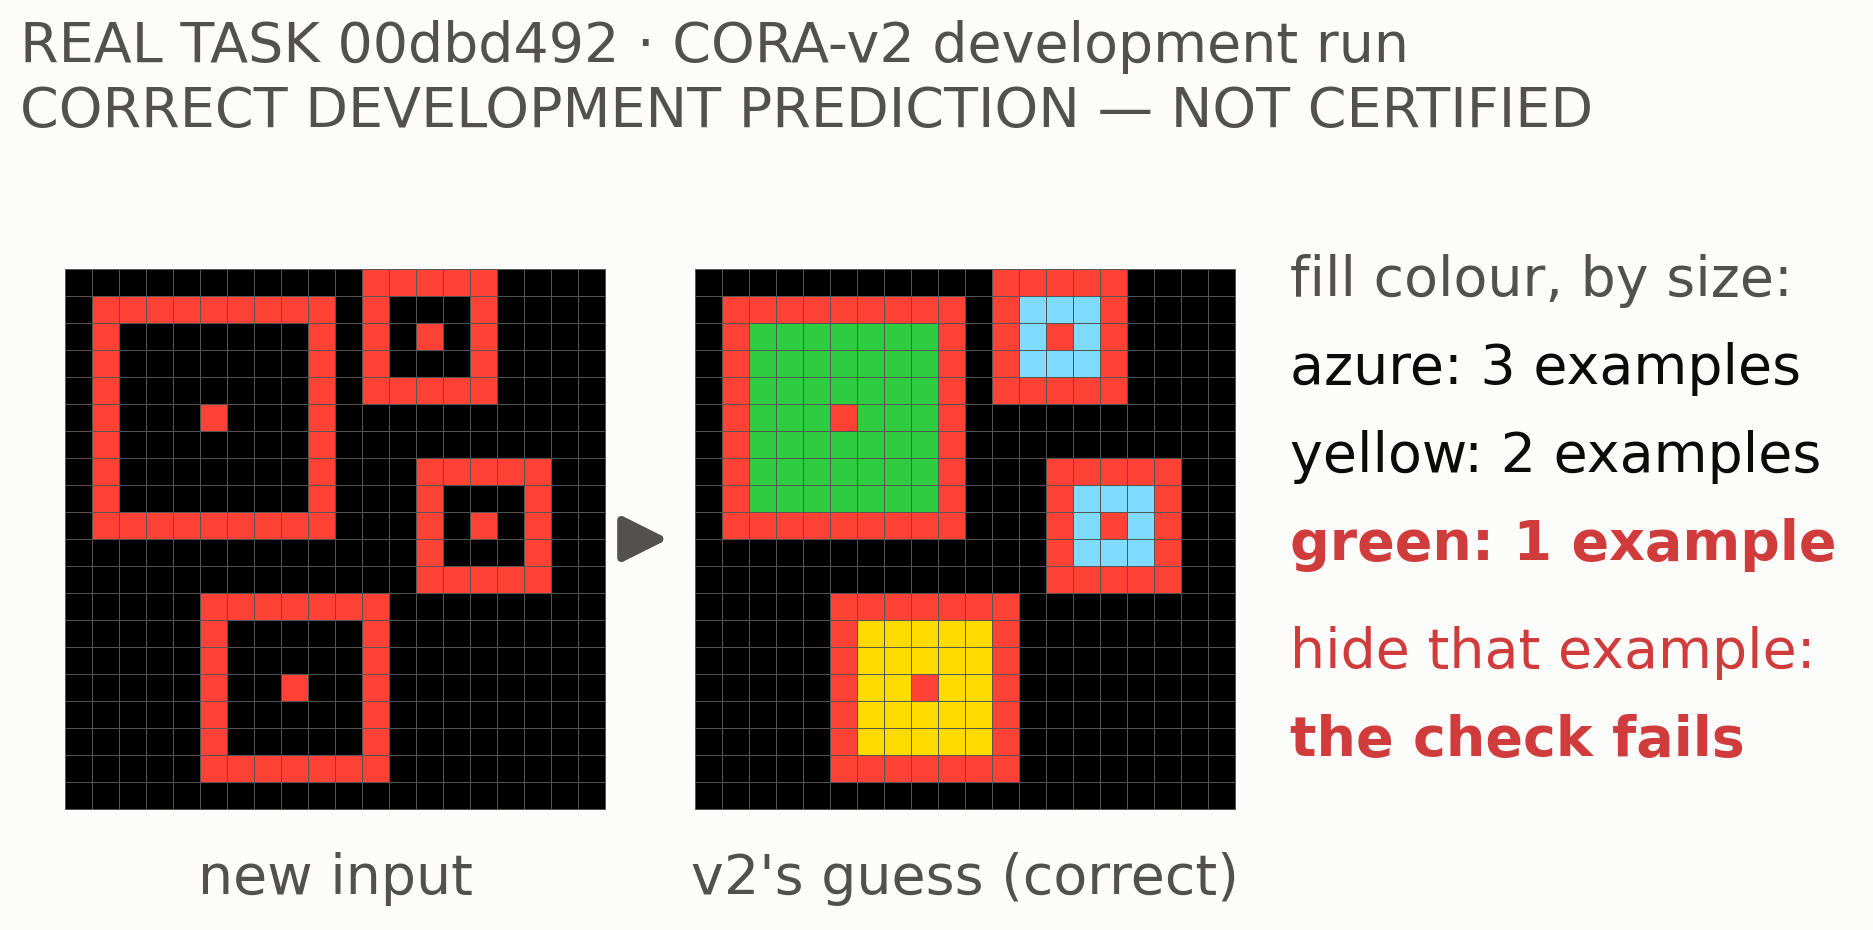
\includegraphics[width=\linewidth]{figures/fig_v2_uncertified_00dbd492_large.png}
  \end{tikzfigure}
  \secfont\color{ink2} 118 exposed tasks: 4 right, 1 wrong guess; none certified.
}
\block{\bt{From ARC to science}\chip{critical}{FUTURE, NOT TESTED}}{\secfont
  \begin{tikzfigure}
  
\begin{tikzpicture}
    \node[stage, text width=6.2cm] (x1) at (0,0) {ARC grids};
    \node[pstage, text width=6.6cm] (x2) at (8.0,0) {learning what to revise};
    \node[pstage, text width=6.2cm] (x3) at (16.0,0) {scientific data};
    \draw[flow] (x1) -- (x2); \draw[flow] (x2) -- (x3);
  \end{tikzpicture}
  \end{tikzfigure}
  Proteins, omics, plant phenotypes: only the revision policy could transfer.
}
\end{columns}

%======================= BOTTOM LINE AND LEGEND (full width)
\block{}{%
  
\begin{tikzpicture}
    \node[anchor=north west, text width=76cm, align=left] (bl) at (0,0) {\fontsize{48}{58}\selectfont\bfseries
      Building a rule is not learning which revision improves an unseen prediction. That is what we test.};
    \node[stage, text width=8.6cm, anchor=north west] (s) at (0,-2.3) {existing, tested};
    \node[pstage, text width=11.8cm, right=0.8cm of s] (d) {proposed, not yet validated};
    \node[right=1.0cm of d, font=\secfont, align=left] {{\color{good}[DONE]} {\color{critical}[NEGATIVE]}
      {\color{warm}[DEVELOPMENT]}\\ {\color{critical}[FUTURE, NOT TESTED]}};
  \end{tikzpicture}
  \par\vspace{0.3em}
  {\fontsize{22}{27}\selectfont\color{ink2}
  Prior work: Popper, DreamCoder, LILO, Model Discovery Agent; failing and revising is not new. Neural baseline:
  NVARC's published method, reproduced. Numbers: \texttt{records/CORA\_SUMMIT\_CLAIM\_LEDGER\_20261017.md} $\cdot$ AI
  coding assistance used $\cdot$ authorship pending review.\par}
}
\end{document}
